\documentclass[11pt]{report}
%default Package
\usepackage{setup} %package personel
\usepackage{pdfpages}
\usepackage[acronym, toc]{glossaries}
\usepackage{hyperref}
\makenoidxglossaries
    \loadglsentries{glossary}


%\usepackage[breakable]{tcolorbox}
%    \usepackage{parskip} % Stop auto-indenting (to mimic markdown behaviour)
    \usepackage{iftex}
    \ifPDFTeX
    	\usepackage[T1]{fontenc}
    	\usepackage{mathpazo}
    \else
    	\usepackage{fontspec}
    \fi

    % Basic figure setup, for now with no caption control since it's done
    % automatically by Pandoc (which extracts ![](path) syntax from Markdown).
    \usepackage{graphicx}
    % Maintain compatibility with old templates. Remove in nbconvert 6.0
    \let\Oldincludegraphics\includegraphics
    % Ensure that by default, figures have no caption (until we provide a
    % proper Figure object with a Caption API and a way to capture that
    % in the conversion process - todo).


    \usepackage{float}
    \floatplacement{figure}{H} % forces figures to be placed at the correct location
    \usepackage{xcolor} % Allow colors to be defined
    \usepackage{enumerate} % Needed for markdown enumerations to work
    \usepackage{geometry} % Used to adjust the document margins
    \usepackage{amsmath} % Equations
    \usepackage{amssymb} % Equations
    \usepackage{textcomp} % defines textquotesingle
    % Hack from http://tex.stackexchange.com/a/47451/13684:
    \AtBeginDocument{%
        \def\PYZsq{\textquotesingle}% Upright quotes in Pygmentized code
    }
    \usepackage{upquote} % Upright quotes for verbatim code
    \usepackage{eurosym} % defines \euro
    \usepackage[mathletters]{ucs} % Extended unicode (utf-8) support
    \usepackage{fancyvrb} % verbatim replacement that allows latex
    \usepackage{grffile} % extends the file name processing of package graphics 
                         % to support a larger range
    \makeatletter % fix for old versions of grffile with XeLaTeX
    \@ifpackagelater{grffile}{2019/11/01}
    {
      % Do nothing on new versions
    }
    {
      \def\Gread@@xetex#1{%
        \IfFileExists{"\Gin@base".bb}%
        {\Gread@eps{\Gin@base.bb}}%
        {\Gread@@xetex@aux#1}%
      }
    }
    \makeatother
    \usepackage[Export]{adjustbox} % Used to constrain images to a maximum size
    \adjustboxset{max size={0.9\linewidth}{0.9\paperheight}}

    % The hyperref package gives us a pdf with properly built
    % internal navigation ('pdf bookmarks' for the table of contents,
    % internal cross-reference links, web links for URLs, etc.)
    \usepackage{hyperref}
    % The default LaTeX title has an obnoxious amount of whitespace. By default,
    % titling removes some of it. It also provides customization options.
    \usepackage{titling}
    \usepackage{longtable} % longtable support required by pandoc >1.10
    \usepackage{booktabs}  % table support for pandoc > 1.12.2
    \usepackage[inline]{enumitem} % IRkernel/repr support (it uses the enumerate* environment)
    \usepackage[normalem]{ulem} % ulem is needed to support strikethroughs (\sout)
                                % normalem makes italics be italics, not underlines
    \usepackage{mathrsfs}
    

    
    % Colors for the hyperref package
    \definecolor{urlcolor}{rgb}{0,.145,.698}
    \definecolor{linkcolor}{rgb}{.71,0.21,0.01}
    \definecolor{citecolor}{rgb}{.12,.54,.11}

    % ANSI colors
    \definecolor{ansi-black}{HTML}{3E424D}
    \definecolor{ansi-black-intense}{HTML}{282C36}
    \definecolor{ansi-red}{HTML}{E75C58}
    \definecolor{ansi-red-intense}{HTML}{B22B31}
    \definecolor{ansi-green}{HTML}{00A250}
    \definecolor{ansi-green-intense}{HTML}{007427}
    \definecolor{ansi-yellow}{HTML}{DDB62B}
    \definecolor{ansi-yellow-intense}{HTML}{B27D12}
    \definecolor{ansi-blue}{HTML}{208FFB}
    \definecolor{ansi-blue-intense}{HTML}{0065CA}
    \definecolor{ansi-magenta}{HTML}{D160C4}
    \definecolor{ansi-magenta-intense}{HTML}{A03196}
    \definecolor{ansi-cyan}{HTML}{60C6C8}
    \definecolor{ansi-cyan-intense}{HTML}{258F8F}
    \definecolor{ansi-white}{HTML}{C5C1B4}
    \definecolor{ansi-white-intense}{HTML}{A1A6B2}
    \definecolor{ansi-default-inverse-fg}{HTML}{FFFFFF}
    \definecolor{ansi-default-inverse-bg}{HTML}{000000}

    % common color for the border for error outputs.
    \definecolor{outerrorbackground}{HTML}{FFDFDF}

    % commands and environments needed by pandoc snippets
    % extracted from the output of `pandoc -s`
    \providecommand{\tightlist}{%
      \setlength{\itemsep}{0pt}\setlength{\parskip}{0pt}}
    \DefineVerbatimEnvironment{Highlighting}{Verbatim}{commandchars=\\\{\}}
    % Add ',fontsize=\small' for more characters per line
    \newenvironment{Shaded}{}{}
    \newcommand{\KeywordTok}[1]{\textcolor[rgb]{0.00,0.44,0.13}{\textbf{{#1}}}}
    \newcommand{\DataTypeTok}[1]{\textcolor[rgb]{0.56,0.13,0.00}{{#1}}}
    \newcommand{\DecValTok}[1]{\textcolor[rgb]{0.25,0.63,0.44}{{#1}}}
    \newcommand{\BaseNTok}[1]{\textcolor[rgb]{0.25,0.63,0.44}{{#1}}}
    \newcommand{\FloatTok}[1]{\textcolor[rgb]{0.25,0.63,0.44}{{#1}}}
    \newcommand{\CharTok}[1]{\textcolor[rgb]{0.25,0.44,0.63}{{#1}}}
    \newcommand{\StringTok}[1]{\textcolor[rgb]{0.25,0.44,0.63}{{#1}}}
    \newcommand{\CommentTok}[1]{\textcolor[rgb]{0.38,0.63,0.69}{\textit{{#1}}}}
    \newcommand{\OtherTok}[1]{\textcolor[rgb]{0.00,0.44,0.13}{{#1}}}
    \newcommand{\AlertTok}[1]{\textcolor[rgb]{1.00,0.00,0.00}{\textbf{{#1}}}}
    \newcommand{\FunctionTok}[1]{\textcolor[rgb]{0.02,0.16,0.49}{{#1}}}
    \newcommand{\RegionMarkerTok}[1]{{#1}}
    \newcommand{\ErrorTok}[1]{\textcolor[rgb]{1.00,0.00,0.00}{\textbf{{#1}}}}
    \newcommand{\NormalTok}[1]{{#1}}
    
    % Additional commands for more recent versions of Pandoc
    \newcommand{\ConstantTok}[1]{\textcolor[rgb]{0.53,0.00,0.00}{{#1}}}
    \newcommand{\SpecialCharTok}[1]{\textcolor[rgb]{0.25,0.44,0.63}{{#1}}}
    \newcommand{\VerbatimStringTok}[1]{\textcolor[rgb]{0.25,0.44,0.63}{{#1}}}
    \newcommand{\SpecialStringTok}[1]{\textcolor[rgb]{0.73,0.40,0.53}{{#1}}}
    \newcommand{\ImportTok}[1]{{#1}}
    \newcommand{\DocumentationTok}[1]{\textcolor[rgb]{0.73,0.13,0.13}{\textit{{#1}}}}
    \newcommand{\AnnotationTok}[1]{\textcolor[rgb]{0.38,0.63,0.69}{\textbf{\textit{{#1}}}}}
    \newcommand{\CommentVarTok}[1]{\textcolor[rgb]{0.38,0.63,0.69}{\textbf{\textit{{#1}}}}}
    \newcommand{\VariableTok}[1]{\textcolor[rgb]{0.10,0.09,0.49}{{#1}}}
    \newcommand{\ControlFlowTok}[1]{\textcolor[rgb]{0.00,0.44,0.13}{\textbf{{#1}}}}
    \newcommand{\OperatorTok}[1]{\textcolor[rgb]{0.40,0.40,0.40}{{#1}}}
    \newcommand{\BuiltInTok}[1]{{#1}}
    \newcommand{\ExtensionTok}[1]{{#1}}
    \newcommand{\PreprocessorTok}[1]{\textcolor[rgb]{0.74,0.48,0.00}{{#1}}}
    \newcommand{\AttributeTok}[1]{\textcolor[rgb]{0.49,0.56,0.16}{{#1}}}
    \newcommand{\InformationTok}[1]{\textcolor[rgb]{0.38,0.63,0.69}{\textbf{\textit{{#1}}}}}
    \newcommand{\WarningTok}[1]{\textcolor[rgb]{0.38,0.63,0.69}{\textbf{\textit{{#1}}}}}
    
    
    % Define a nice break command that doesn't care if a line doesn't already
    % exist.
    \def\br{\hspace*{\fill} \\* }
    % Math Jax compatibility definitions
    \def\gt{>}
    \def\lt{<}
    \let\Oldtex\TeX
    \let\Oldlatex\LaTeX
    \renewcommand{\TeX}{\textrm{\Oldtex}}
    \renewcommand{\LaTeX}{\textrm{\Oldlatex}}
    % Document parameters
    % Document title

    
    
    
    
% Pygments definitions
\makeatletter
\def\PY@reset{\let\PY@it=\relax \let\PY@bf=\relax%
    \let\PY@ul=\relax \let\PY@tc=\relax%
    \let\PY@bc=\relax \let\PY@ff=\relax}
\def\PY@tok#1{\csname PY@tok@#1\endcsname}
\def\PY@toks#1+{\ifx\relax#1\empty\else%
    \PY@tok{#1}\expandafter\PY@toks\fi}
\def\PY@do#1{\PY@bc{\PY@tc{\PY@ul{%
    \PY@it{\PY@bf{\PY@ff{#1}}}}}}}
\def\PY#1#2{\PY@reset\PY@toks#1+\relax+\PY@do{#2}}

\@namedef{PY@tok@w}{\def\PY@tc##1{\textcolor[rgb]{0.73,0.73,0.73}{##1}}}
\@namedef{PY@tok@c}{\let\PY@it=\textit\def\PY@tc##1{\textcolor[rgb]{0.25,0.50,0.50}{##1}}}
\@namedef{PY@tok@cp}{\def\PY@tc##1{\textcolor[rgb]{0.74,0.48,0.00}{##1}}}
\@namedef{PY@tok@k}{\let\PY@bf=\textbf\def\PY@tc##1{\textcolor[rgb]{0.00,0.50,0.00}{##1}}}
\@namedef{PY@tok@kp}{\def\PY@tc##1{\textcolor[rgb]{0.00,0.50,0.00}{##1}}}
\@namedef{PY@tok@kt}{\def\PY@tc##1{\textcolor[rgb]{0.69,0.00,0.25}{##1}}}
\@namedef{PY@tok@o}{\def\PY@tc##1{\textcolor[rgb]{0.40,0.40,0.40}{##1}}}
\@namedef{PY@tok@ow}{\let\PY@bf=\textbf\def\PY@tc##1{\textcolor[rgb]{0.67,0.13,1.00}{##1}}}
\@namedef{PY@tok@nb}{\def\PY@tc##1{\textcolor[rgb]{0.00,0.50,0.00}{##1}}}
\@namedef{PY@tok@nf}{\def\PY@tc##1{\textcolor[rgb]{0.00,0.00,1.00}{##1}}}
\@namedef{PY@tok@nc}{\let\PY@bf=\textbf\def\PY@tc##1{\textcolor[rgb]{0.00,0.00,1.00}{##1}}}
\@namedef{PY@tok@nn}{\let\PY@bf=\textbf\def\PY@tc##1{\textcolor[rgb]{0.00,0.00,1.00}{##1}}}
\@namedef{PY@tok@ne}{\let\PY@bf=\textbf\def\PY@tc##1{\textcolor[rgb]{0.82,0.25,0.23}{##1}}}
\@namedef{PY@tok@nv}{\def\PY@tc##1{\textcolor[rgb]{0.10,0.09,0.49}{##1}}}
\@namedef{PY@tok@no}{\def\PY@tc##1{\textcolor[rgb]{0.53,0.00,0.00}{##1}}}
\@namedef{PY@tok@nl}{\def\PY@tc##1{\textcolor[rgb]{0.63,0.63,0.00}{##1}}}
\@namedef{PY@tok@ni}{\let\PY@bf=\textbf\def\PY@tc##1{\textcolor[rgb]{0.60,0.60,0.60}{##1}}}
\@namedef{PY@tok@na}{\def\PY@tc##1{\textcolor[rgb]{0.49,0.56,0.16}{##1}}}
\@namedef{PY@tok@nt}{\let\PY@bf=\textbf\def\PY@tc##1{\textcolor[rgb]{0.00,0.50,0.00}{##1}}}
\@namedef{PY@tok@nd}{\def\PY@tc##1{\textcolor[rgb]{0.67,0.13,1.00}{##1}}}
\@namedef{PY@tok@s}{\def\PY@tc##1{\textcolor[rgb]{0.73,0.13,0.13}{##1}}}
\@namedef{PY@tok@sd}{\let\PY@it=\textit\def\PY@tc##1{\textcolor[rgb]{0.73,0.13,0.13}{##1}}}
\@namedef{PY@tok@si}{\let\PY@bf=\textbf\def\PY@tc##1{\textcolor[rgb]{0.73,0.40,0.53}{##1}}}
\@namedef{PY@tok@se}{\let\PY@bf=\textbf\def\PY@tc##1{\textcolor[rgb]{0.73,0.40,0.13}{##1}}}
\@namedef{PY@tok@sr}{\def\PY@tc##1{\textcolor[rgb]{0.73,0.40,0.53}{##1}}}
\@namedef{PY@tok@ss}{\def\PY@tc##1{\textcolor[rgb]{0.10,0.09,0.49}{##1}}}
\@namedef{PY@tok@sx}{\def\PY@tc##1{\textcolor[rgb]{0.00,0.50,0.00}{##1}}}
\@namedef{PY@tok@m}{\def\PY@tc##1{\textcolor[rgb]{0.40,0.40,0.40}{##1}}}
\@namedef{PY@tok@gh}{\let\PY@bf=\textbf\def\PY@tc##1{\textcolor[rgb]{0.00,0.00,0.50}{##1}}}
\@namedef{PY@tok@gu}{\let\PY@bf=\textbf\def\PY@tc##1{\textcolor[rgb]{0.50,0.00,0.50}{##1}}}
\@namedef{PY@tok@gd}{\def\PY@tc##1{\textcolor[rgb]{0.63,0.00,0.00}{##1}}}
\@namedef{PY@tok@gi}{\def\PY@tc##1{\textcolor[rgb]{0.00,0.63,0.00}{##1}}}
\@namedef{PY@tok@gr}{\def\PY@tc##1{\textcolor[rgb]{1.00,0.00,0.00}{##1}}}
\@namedef{PY@tok@ge}{\let\PY@it=\textit}
\@namedef{PY@tok@gs}{\let\PY@bf=\textbf}
\@namedef{PY@tok@gp}{\let\PY@bf=\textbf\def\PY@tc##1{\textcolor[rgb]{0.00,0.00,0.50}{##1}}}
\@namedef{PY@tok@go}{\def\PY@tc##1{\textcolor[rgb]{0.53,0.53,0.53}{##1}}}
\@namedef{PY@tok@gt}{\def\PY@tc##1{\textcolor[rgb]{0.00,0.27,0.87}{##1}}}
\@namedef{PY@tok@err}{\def\PY@bc##1{{\setlength{\fboxsep}{\string -\fboxrule}\fcolorbox[rgb]{1.00,0.00,0.00}{1,1,1}{\strut ##1}}}}
\@namedef{PY@tok@kc}{\let\PY@bf=\textbf\def\PY@tc##1{\textcolor[rgb]{0.00,0.50,0.00}{##1}}}
\@namedef{PY@tok@kd}{\let\PY@bf=\textbf\def\PY@tc##1{\textcolor[rgb]{0.00,0.50,0.00}{##1}}}
\@namedef{PY@tok@kn}{\let\PY@bf=\textbf\def\PY@tc##1{\textcolor[rgb]{0.00,0.50,0.00}{##1}}}
\@namedef{PY@tok@kr}{\let\PY@bf=\textbf\def\PY@tc##1{\textcolor[rgb]{0.00,0.50,0.00}{##1}}}
\@namedef{PY@tok@bp}{\def\PY@tc##1{\textcolor[rgb]{0.00,0.50,0.00}{##1}}}
\@namedef{PY@tok@fm}{\def\PY@tc##1{\textcolor[rgb]{0.00,0.00,1.00}{##1}}}
\@namedef{PY@tok@vc}{\def\PY@tc##1{\textcolor[rgb]{0.10,0.09,0.49}{##1}}}
\@namedef{PY@tok@vg}{\def\PY@tc##1{\textcolor[rgb]{0.10,0.09,0.49}{##1}}}
\@namedef{PY@tok@vi}{\def\PY@tc##1{\textcolor[rgb]{0.10,0.09,0.49}{##1}}}
\@namedef{PY@tok@vm}{\def\PY@tc##1{\textcolor[rgb]{0.10,0.09,0.49}{##1}}}
\@namedef{PY@tok@sa}{\def\PY@tc##1{\textcolor[rgb]{0.73,0.13,0.13}{##1}}}
\@namedef{PY@tok@sb}{\def\PY@tc##1{\textcolor[rgb]{0.73,0.13,0.13}{##1}}}
\@namedef{PY@tok@sc}{\def\PY@tc##1{\textcolor[rgb]{0.73,0.13,0.13}{##1}}}
\@namedef{PY@tok@dl}{\def\PY@tc##1{\textcolor[rgb]{0.73,0.13,0.13}{##1}}}
\@namedef{PY@tok@s2}{\def\PY@tc##1{\textcolor[rgb]{0.73,0.13,0.13}{##1}}}
\@namedef{PY@tok@sh}{\def\PY@tc##1{\textcolor[rgb]{0.73,0.13,0.13}{##1}}}
\@namedef{PY@tok@s1}{\def\PY@tc##1{\textcolor[rgb]{0.73,0.13,0.13}{##1}}}
\@namedef{PY@tok@mb}{\def\PY@tc##1{\textcolor[rgb]{0.40,0.40,0.40}{##1}}}
\@namedef{PY@tok@mf}{\def\PY@tc##1{\textcolor[rgb]{0.40,0.40,0.40}{##1}}}
\@namedef{PY@tok@mh}{\def\PY@tc##1{\textcolor[rgb]{0.40,0.40,0.40}{##1}}}
\@namedef{PY@tok@mi}{\def\PY@tc##1{\textcolor[rgb]{0.40,0.40,0.40}{##1}}}
\@namedef{PY@tok@il}{\def\PY@tc##1{\textcolor[rgb]{0.40,0.40,0.40}{##1}}}
\@namedef{PY@tok@mo}{\def\PY@tc##1{\textcolor[rgb]{0.40,0.40,0.40}{##1}}}
\@namedef{PY@tok@ch}{\let\PY@it=\textit\def\PY@tc##1{\textcolor[rgb]{0.25,0.50,0.50}{##1}}}
\@namedef{PY@tok@cm}{\let\PY@it=\textit\def\PY@tc##1{\textcolor[rgb]{0.25,0.50,0.50}{##1}}}
\@namedef{PY@tok@cpf}{\let\PY@it=\textit\def\PY@tc##1{\textcolor[rgb]{0.25,0.50,0.50}{##1}}}
\@namedef{PY@tok@c1}{\let\PY@it=\textit\def\PY@tc##1{\textcolor[rgb]{0.25,0.50,0.50}{##1}}}
\@namedef{PY@tok@cs}{\let\PY@it=\textit\def\PY@tc##1{\textcolor[rgb]{0.25,0.50,0.50}{##1}}}

\def\PYZbs{\char`\\}
\def\PYZus{\char`\_}
\def\PYZob{\char`\{}
\def\PYZcb{\char`\}}
\def\PYZca{\char`\^}
\def\PYZam{\char`\&}
\def\PYZlt{\char`\<}
\def\PYZgt{\char`\>}
\def\PYZsh{\char`\#}
\def\PYZpc{\char`\%}
\def\PYZdl{\char`\$}
\def\PYZhy{\char`\-}
\def\PYZsq{\char`\'}
\def\PYZdq{\char`\"}
\def\PYZti{\char`\~}
% for compatibility with earlier versions
\def\PYZat{@}
\def\PYZlb{[}
\def\PYZrb{]}
\makeatother


    % For linebreaks inside Verbatim environment from package fancyvrb. 
    \makeatletter
        \newbox\Wrappedcontinuationbox 
        \newbox\Wrappedvisiblespacebox 
        \newcommand*\Wrappedvisiblespace {\textcolor{red}{\textvisiblespace}} 
        \newcommand*\Wrappedcontinuationsymbol {\textcolor{red}{\llap{\tiny$\m@th\hookrightarrow$}}} 
        \newcommand*\Wrappedcontinuationindent {3ex } 
        \newcommand*\Wrappedafterbreak {\kern\Wrappedcontinuationindent\copy\Wrappedcontinuationbox} 
        % Take advantage of the already applied Pygments mark-up to insert 
        % potential linebreaks for TeX processing. 
        %        {, <, #, %, $, ' and ": go to next line. 
        %        _, }, ^, &, >, - and ~: stay at end of broken line. 
        % Use of \textquotesingle for straight quote. 
        \newcommand*\Wrappedbreaksatspecials {% 
            \def\PYGZus{\discretionary{\char`\_}{\Wrappedafterbreak}{\char`\_}}% 
            \def\PYGZob{\discretionary{}{\Wrappedafterbreak\char`\{}{\char`\{}}% 
            \def\PYGZcb{\discretionary{\char`\}}{\Wrappedafterbreak}{\char`\}}}% 
            \def\PYGZca{\discretionary{\char`\^}{\Wrappedafterbreak}{\char`\^}}% 
            \def\PYGZam{\discretionary{\char`\&}{\Wrappedafterbreak}{\char`\&}}% 
            \def\PYGZlt{\discretionary{}{\Wrappedafterbreak\char`\<}{\char`\<}}% 
            \def\PYGZgt{\discretionary{\char`\>}{\Wrappedafterbreak}{\char`\>}}% 
            \def\PYGZsh{\discretionary{}{\Wrappedafterbreak\char`\#}{\char`\#}}% 
            \def\PYGZpc{\discretionary{}{\Wrappedafterbreak\char`\%}{\char`\%}}% 
            \def\PYGZdl{\discretionary{}{\Wrappedafterbreak\char`\$}{\char`\$}}% 
            \def\PYGZhy{\discretionary{\char`\-}{\Wrappedafterbreak}{\char`\-}}% 
            \def\PYGZsq{\discretionary{}{\Wrappedafterbreak\textquotesingle}{\textquotesingle}}% 
            \def\PYGZdq{\discretionary{}{\Wrappedafterbreak\char`\"}{\char`\"}}% 
            \def\PYGZti{\discretionary{\char`\~}{\Wrappedafterbreak}{\char`\~}}% 
        } 
        % Some characters . , ; ? ! / are not pygmentized. 
        % This macro makes them "active" and they will insert potential linebreaks 
        \newcommand*\Wrappedbreaksatpunct {% 
            \lccode`\~`\.\lowercase{\def~}{\discretionary{\hbox{\char`\.}}{\Wrappedafterbreak}{\hbox{\char`\.}}}% 
            \lccode`\~`\,\lowercase{\def~}{\discretionary{\hbox{\char`\,}}{\Wrappedafterbreak}{\hbox{\char`\,}}}% 
            \lccode`\~`\;\lowercase{\def~}{\discretionary{\hbox{\char`\;}}{\Wrappedafterbreak}{\hbox{\char`\;}}}% 
            \lccode`\~`\:\lowercase{\def~}{\discretionary{\hbox{\char`\:}}{\Wrappedafterbreak}{\hbox{\char`\:}}}% 
            \lccode`\~`\?\lowercase{\def~}{\discretionary{\hbox{\char`\?}}{\Wrappedafterbreak}{\hbox{\char`\?}}}% 
            \lccode`\~`\!\lowercase{\def~}{\discretionary{\hbox{\char`\!}}{\Wrappedafterbreak}{\hbox{\char`\!}}}% 
            \lccode`\~`\/\lowercase{\def~}{\discretionary{\hbox{\char`\/}}{\Wrappedafterbreak}{\hbox{\char`\/}}}% 
            \catcode`\.\active
            \catcode`\,\active 
            \catcode`\;\active
            \catcode`\:\active
            \catcode`\?\active
            \catcode`\!\active
            \catcode`\/\active 
            \lccode`\~`\~ 	
        }
    \makeatother

    \let\OriginalVerbatim=\Verbatim
    \makeatletter
    \renewcommand{\Verbatim}[1][1]{%
        %\parskip\z@skip
        \sbox\Wrappedcontinuationbox {\Wrappedcontinuationsymbol}%
        \sbox\Wrappedvisiblespacebox {\FV@SetupFont\Wrappedvisiblespace}%
        \def\FancyVerbFormatLine ##1{\hsize\linewidth
            \vtop{\raggedright\hyphenpenalty\z@\exhyphenpenalty\z@
                \doublehyphendemerits\z@\finalhyphendemerits\z@
                \strut ##1\strut}%
        }%
        % If the linebreak is at a space, the latter will be displayed as visible
        % space at end of first line, and a continuation symbol starts next line.
        % Stretch/shrink are however usually zero for typewriter font.
        \def\FV@Space {%
            \nobreak\hskip\z@ plus\fontdimen3\font minus\fontdimen4\font
            \discretionary{\copy\Wrappedvisiblespacebox}{\Wrappedafterbreak}
            {\kern\fontdimen2\font}%
        }%
        
        % Allow breaks at special characters using \PYG... macros.
        \Wrappedbreaksatspecials
        % Breaks at punctuation characters . , ; ? ! and / need catcode=\active 	
        \OriginalVerbatim[#1,codes*=\Wrappedbreaksatpunct]%
    }
    \makeatother

    % Exact colors from NB
    \definecolor{incolor}{HTML}{303F9F}
    \definecolor{outcolor}{HTML}{D84315}
    \definecolor{cellborder}{HTML}{CFCFCF}
    \definecolor{cellbackground}{HTML}{F7F7F7}
    
    % prompt
    \makeatletter
    \newcommand{\boxspacing}{\kern\kvtcb@left@rule\kern\kvtcb@boxsep}
    \makeatother
    \newcommand{\prompt}[4]{
        {\ttfamily\llap{{\color{#2}[#3]:\hspace{3pt}#4}}\vspace{-\baselineskip}}
    }
    

    
    % Prevent overflowing lines due to hard-to-break entities
    \sloppy 

    
    \geometry{verbose,tmargin=1in,bmargin=1in,lmargin=1in,rmargin=1in}

\begin{document}
    % Renommer les listings
    \renewcommand\lstlistingname{Code}
    \renewcommand\lstlistlistingname{Liste des codes}

    %afficher la page de garde
    \newgeometry{left=2.5cm, right=2.5cm, top=3cm, bottom=2.5cm}
\newcommand{\HRule}{\rule{\linewidth}{0.5mm}}

\begingroup
    \centering
    \begin{titlepage}
        
\includegraphics[width=400px]{images/logo_heia-fr.png}
        \vspace{1.5cm}
        
        {\scshape\LARGE\bfseries Plugin IntelliJ pour GNU Prolog } \\[0.5cm]
        {\scshape\Large Projet de semestre 5}\\[0.5cm]
        {\scshape\Large 2022 - 2023}\\[1cm]
        
        \HRule \\[0.4cm]
        \vspace{0.8cm}
        {\Huge\bfseries Rapport}\\[0.5cm]
        \vspace{0.3cm}
        \HRule \\[.5cm]
        {\scshape STURZENEGGER Erwan}\\[0.5cm]
        {\scshape ISC-IL-3}\\[0.3cm]
        \HRule \\[0.5cm]
        
        \begin{flushleft}
            \large
        	{\bfseries Mandant :}\\
        	Bapst Frédéric
        	\vspace{2em}	
        \end{flushleft}
        
        \begin{flushleft}
            \large
        	{\bfseries Superviseur :}\\
        	Bapst Frédéric
        	\vspace{1em}	
        \end{flushleft}
        
        \vfill
        \centering{\large \today}\\	
    \end{titlepage}
\endgroup
\restoregeometry
    \pagenumbering{Roman}
    \pagestyle{fancy} %mettre l'entête pour les pages suivantes
    % table of contents
    \renewcommand*\contentsname{Table des matières}
    \tableofcontents

    % table of tables
    \clearpage
    \pagenumbering{arabic}
    
    % Introduction
    % ==========================================================================================================
%                                               INTRODUCTION
% ==========================================================================================================

\chapter{Introduction}
\noindent
Ce document est le rapport du projet de semestre 5 : \textit{Plugin IntelliJ pour GNU-Prolog}.
Il a pour but de permettre la compréhension des différentes étapes de la réalisation du projet et du fonctionnement du plugin.

\section{Contexte}
\noindent
Dans le cadre d’un projet de semestre (printemps 2018), un plugin IntelliJ-IDEA a été réalisé, permettant ainsi d’aider les étudiants lors du développement de programmes Gnu-Prolog.
Actuellement, le plugin est employé en 3ème année pour le cours de programmation logique.
Bien que fonctionnel, il n’est pas parfait et n’offre pas certaines fonctions qui seraient très utiles. En outre, un bug
ne permet pas aux utilisateurs du plugin travaillant sur Windows de lancer l’exécution du programme directement dans le terminal de l’IDE.

\section{Motivations}
\noindent
Mes motivations à prendre ce projet sont multiples :
\begin{itemize}
    \item \textbf{Apprentissage :} J'ai très envie de découvrir le fonctionnement d'un plugin IntelliJ, et de voir comment il est possible de créer un plugin pour un IDE.
    \item \textbf{Utilité :} Le plugin sera utilisé par les étudiants de 3ème années de la filière ISC, spécialisé dans l'informatique logicielle.
    \item \textbf{Projet :} Le projet étant déjà existant, je devrai m'adapter à son fonctionnement et le faire évoluer.
\end{itemize}

\section{Objectifs}
\subsection{Mise à jour du plugin}
\noindent
Le premier objectif est de mettre à jour le plugin afin qu'il soit compatible avec les dernières versions d'IntelliJ. En effet, le plugin a été développé en 2018, et n'est plus compatible avec les dernières versions du SDK d'IntelliJ. Il est donc nécessaire de mettre à jour le plugin afin d'éviter une perte de compatibilité avec les futures versions d'IntelliJ.
\\ Ceci comprendra :
\begin{itemize}
    \item \textbf{Passage du projet sur Gradle}: Le plugin a été développé sans aucune gestion de dépendances, et utilise un système de librairies externes. Il est donc nécessaire de passer le projet sur Gradle afin de gérer les dépendances.
    \item \textbf{Mise à jour des dépendances}: Changement de la version du SDK d'IntelliJ, mise à jour des dépendances du plugin.
    \item \textbf{Mise à jour du code}: Mise à jour des classes et méthodes dépréciées.
    \item \textbf{Corrections des bugs}: Correction des bugs qui empêchent le plugin de fonctionner correctement.
    \item \textbf{Implémentation des tests unitaires}: Implémentation des tests unitaires pour le plugin.
    \item \textbf{Mise en place d'une pipeline}: Mise en place d'une pipeline pour effectuer les tests unitaires et la compilation du plugin.
\end{itemize}
\subsection{Ajout de fonctionnalités}
\noindent
Le second objectif est d'ajouter des fonctionnalités au plugin. En effet, le plugin actuel ne permet pas de faire certaines actions qui seraient très utiles pour les étudiants.
\\ Ces fonctionnalités sont :
\begin{itemize}
    \item \textbf{Navigation}: Ajout de la navigation vers les définitions des prédicats et vers leur usage dans le projet.
    \item \textbf{Refactoring}: Ajout de la possibilité de renommer les prédicats et les variables.
    \item \textbf{Autocomplétion}: Ajout de l'autocomplétion des prédicats et des variables.
    \item \textbf{Affichage des erreurs et des warnings}: Ajout de l'affichage des erreurs et des warnings dans le code.
    \item \textbf{Formatage du code}: Ajout de la possibilité de formater le code.
    \item \textbf{Déploiement du plugin}: Déploiement du plugin sur le marketplace d'IntelliJ et sur le site de GNU-Prolog.
\end{itemize}

\section{Structure du rapport}
\noindent
Ce rapport est divisé en 4 grandes parties :
\begin{itemize}
    \item \textbf{Introduction}: Présentation du projet et de ses objectifs.
    \item \textbf{Mise à jour du plugin}: Présentation de la mise à jour du plugin, de la correction des bugs et de l'ajout des tests unitaires.
    \item \textbf{Ajout des fonctionnalités}: Présentation de l'ajout des fonctionnalités au plugin.
    \item \textbf{Conclusion}: Conclusion du projet.
\end{itemize}
    \chapter{Mise à jour du Plugin}



\noindent
Ce chapitre traite de la correction des bugs existants dans le plugin, de la mise à jour du SDK ainsi que le remplacement des méthodes dépréciées par des méthodes plus récentes.
Enfin, un pipeline a été mis en place sur GitLab afin de tester le plugin à chaque commit.


\section{Correction des bugs}
\noindent Les bugs existants identifiés dans le plugin sont les suivants :

\begin{itemize}
    \item \textbf{Bug 1 :} Le plugin ne permet pas de lancer le script prolog dans la console d'IntelliJ Idea sous Windows.
    \item \textbf{Bug 2 :} Le plugin ne reconnaît pas un opérateur lors de la programmation logique par contrainte.
\end{itemize}

\subsection{Bug 1 : Run dans la console d'IntelliJ Idea sous Windows}
\noindent
Le plugin ne permet pas de lancer le script prolog dans la console d'IntelliJ Idea sous Windows.
\\
\\
\textbf{Description du bug}: Une fois le script prolog compilé et lancé, l'interpréteur prolog boucle sur l'entrée de la console d'IntelliJ Idea, ce qui empêche l'utilisateur de saisir des commandes.
\\
\begin{figure}
    \centering
    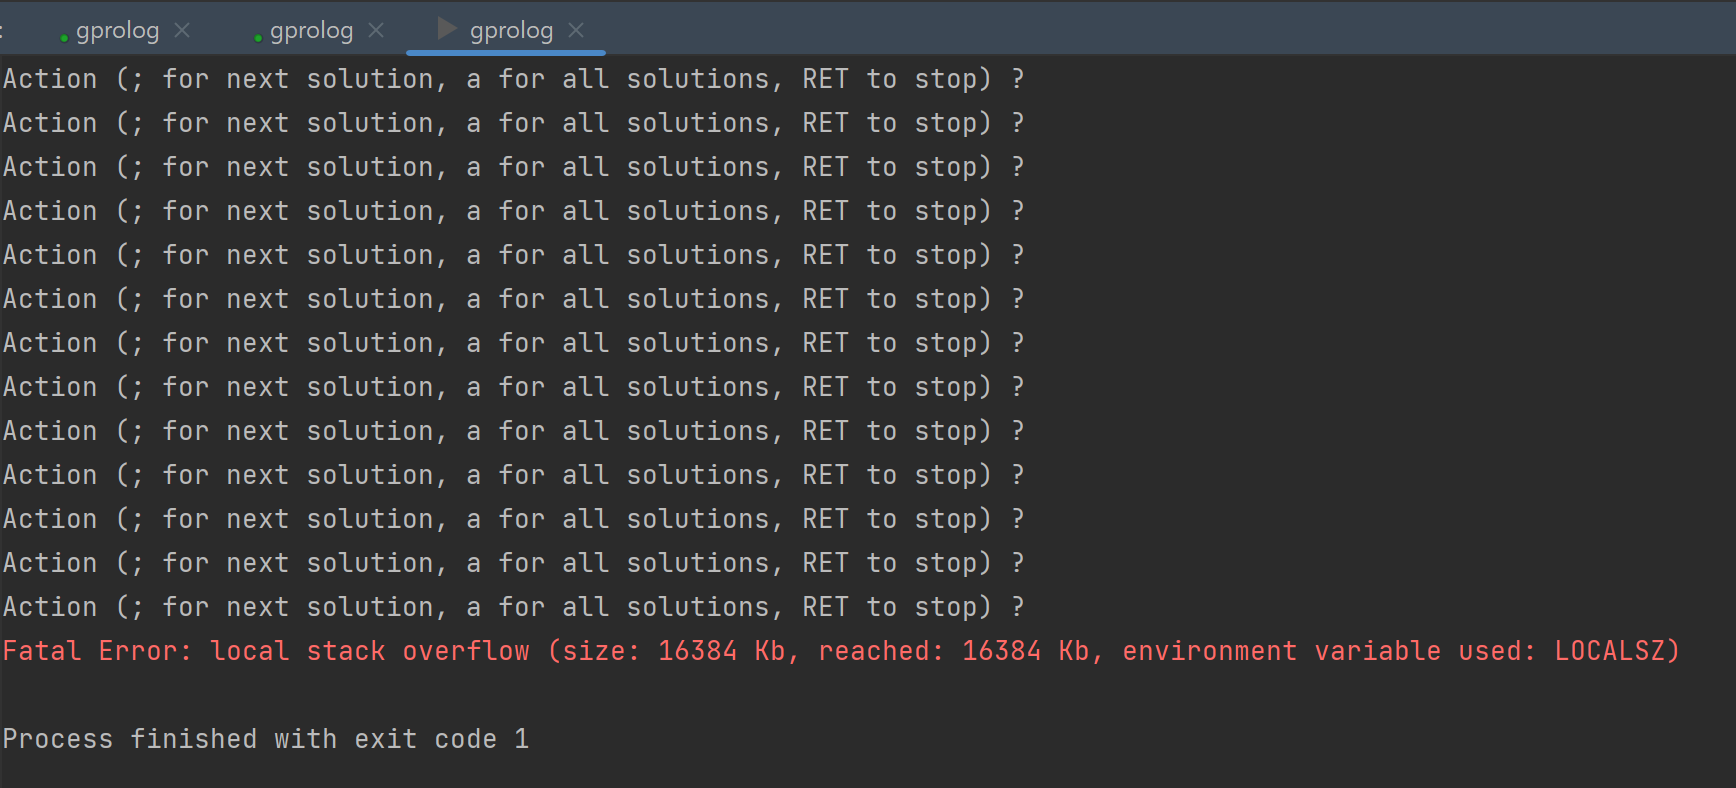
\includegraphics[scale=.85]{images/Bug_1_Windows.png}
    \caption{Image du bug en action dans la console d'IntelliJ Idea}
    \label{fig:bug_1_windows}
\end{figure}

\noindent \textbf{Cause du bug}: La cause n'a pas été clairement identifiée. Cependant, il semble que le problème vienne du fait que le programme prolog s'attend à recevoir des entrées de la console d'IntelliJ Idea et que celle-ci lui envoie des retours à la ligne sans que l'utilisateur ne les ait saisis. Malgré plusieurs tests, je n'ai pas réussi à trouver la cause exacte du problème.
\\
Comme le problème ne se pose pas sous Linux et macOS, il est possible que celui-ci vienne de la façon dont IntelliJ Idea gère les retours à la ligne sous Windows.
\\
Un test à envisager serait de faire notre propre programme qui attend des entrées de la console et de voir si le problème se pose également. Si c'est le cas, alors le problème ne vient pas du plugin mais d'IntelliJ Idea. Si le problème ne se pose pas, alors il faudrait en chercher la cause dans le plugin ou dans l'interpréteur prolog.
\\
\\
\textbf{Solution du bug}: Durant l'implémentation de la fonctionnalité permettant d'afficher les erreurs de compilation dans le code, j'ai trouvé une solution fonctionnelle.
\newdoubleline En lançant une invite de commande invisible, il est possible de lancer des commandes via les InputStream et OutputStream de Java. Voici le code permettant de lancer le script prolog :
\begin{lstlisting}[caption={Code permettant de lancer le script prolog}, label={lst:run_script_prolog}]
private Process createWindowsProcess(Path interpreterPath) throws IOException {
    Process p;
    BufferedWriter writer;
    command = "cmd.exe /min";

    if (isInExternalWindow) {
        p = Runtime.getRuntime().exec("cmd.exe /min");
        writer = new BufferedWriter(new OutputStreamWriter(p.getOutputStream()));
        writer.write("cd " + Path.of(getWorkingDir())); //Go to the working directory
        writer.newLine();
        writer.write("set LINEDIT=gui=yes"); //Prevent windows from opening a console
        writer.newLine();
        String query = " --query-goal \"consult('" + Path.of(filePath).getFileName() + "')\"";
        writer.write("start " + interpreterPath.toString() + query); //Launch the compiler
        writer.newLine();
    } else {
        p = Runtime.getRuntime().exec("cmd.exe /min");
        writer = new BufferedWriter(new OutputStreamWriter(p.getOutputStream()));
        writer.write("set LINEDIT=gui=no"); //Prevent windows from opening a console
        writer.newLine();
        writer.write("cd " + Path.of(getWorkingDir())); //Go to the working directory
        writer.newLine();
        writer.write(interpreterPath.toString()); //Launch the compiler
        writer.newLine();
        writer.write("consult('" + Path.of(filePath).getFileName() + "').");
        writer.newLine();
    }

    writer.flush();

    return p;
}
\end{lstlisting}

\subsection{Bug 2 : Opérateur non reconnu lors de la PLC}
\noindent Le plugin ne reconnaît pas un opérateur lors de la programmation logique par contrainte.
\\
\\
\textbf{Description du bug}: L'opérateur "\#=<" n'est pas reconnu en temps que réel opérateur.
\\
\begin{figure}
    \centering
    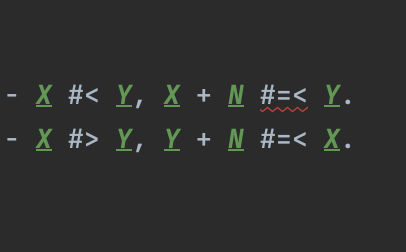
\includegraphics[scale=.85]{images/PLC_error.png}
    \caption{Image du bug en action dans l'éditeur}
    \label{fig:bug_2_plc_op}
\end{figure}

\noindent \textbf{Cause du bug}: Dans le fichier de grammaire BNF, l'opérateur "\#=<" n'est pas présent mais, à la place, il y a l'opérateur "\#<=" qui, lui, n'existe pas en Prolog.
Il s'agit certainement d'une faute de frappe lors de la rédaction de celui-ci.
\\
\textbf{Solution du bug}: L'opérateur a été ajouté dans la grammaire.

\section{Mise à jour du SDK}
\noindent
Le SDK utilisé pour le développement du plugin est la version 173.0 (2017.3.xxx) de IntelliJ Idea.
Actuellement, la version la plus récente est la 222.4345.14 (2022.2.3) et de nombreuses méthodes utilisées dans le plugin sont dépréciées.
\newdoubleline Le but est de mettre à jour le SDK vers une version plus récente afin de pouvoir utiliser les méthodes les plus récentes.

\subsection{Passage du projet en Gradle}
\noindent
Le projet existant n'avait aucun gestionnaire de dépendances et les dépendances étaient gérées manuellement.
Pour lancer le plugin, il fallait donc installer un IDE (par exemple IntelliJ Idea Community) et ajouter les dépendances dans les paramètres du projet.
\\ \noindent Afin de se conformer à la documentation de JetBrains ainsi que de faciliter grandement le développement du plugin, le projet a été migré vers Gradle.
\\\noindent Pour cela, il a fallu ajouter un fichier build.gradle.kts à la racine du projet et configurer les dépendances.
\\ \noindent Afin de pouvoir générer le parser et le lexer, il a fallu ajouter des goals Gradle pour lancer les commandes suivantes :
\begin{lstlisting}[caption={Génération du parser et du lexer}, label={lst:gen_parser_lexer}]
gradle generateParser
gradle generateLexer
\end{lstlisting}


\noindent Ces commandes sont définies dans le fichier build.gradle.kts et permettent de générer le parser et le lexer à partir des fichiers .flex et .bnf.
\begin{lstlisting}[caption={Gradle pour la génération du parser et du lexer}, label={lst:gradle_lexer_parser}]
generateLexer {
    source.set("src/main/java/ch/heiafr/intelliprolog/Prolog.flex")
    targetDir.set("src/gen/java/ch/heiafr/intelliprolog/")
    targetClass.set("PrologLexer")
    skeleton.set(file("src/main/java/ch/heiafr/intelliprolog/Prolog.skeleton"))
    purgeOldFiles.set(true)
}


generateParser {

    try {
        val compiledFilesSources =
            files("build/classes/java/main/")
        classpath.from(compiledFilesSources)
    } catch (e: Exception) {
        // Ignore => no compiled files when running the task for the first time
    }

    source.set("src/main/java/ch/heiafr/intelliprolog/Prolog.bnf")
    targetRoot.set("src/gen/java/")
    pathToParser.set("PrologParser.java")
    pathToPsiRoot.set("psi")
    purgeOldFiles.set(false)
}
\end{lstlisting}
\noindent Il a aussi fallu configurer le GrammarKit afin de spécifier la version de JFlex.

\begin{lstlisting}[caption={Utilisation de JFlex}, label={lst:jflex}]
grammarKit {
    jflexRelease.set("1.7.0-2")
}
\end{lstlisting}

Un fichier settings.properties a également été ajouté afin de spécifier :
\begin{itemize}
    \item Le nom du plugin
    \item Le groupe du plugin
    \item La version du plugin
    \item La version minimum d'IntelliJ Idea requise pour lancer le plugin
    \item La plateforme cible (Ultimate, Education, Community) pour lancer le plugin
    \item La version de la plateforme cible pour lancer le plugin
    \item La dépendance de la plateforme cible
    \item La version de Java utilisée
    \item La version cible de Java pour le Kotlin
    \item La version de Gradle utilisée
\end{itemize}

Le fichier settings.properties est lu par le fichier build.gradle.kts afin de configurer le plugin lors de la compilation ainsi que lors de la création du ZIP du plugin.

\subsection{Le problème du GrammarKit}
\noindent
Le plugin utilise le GrammarKit afin de générer le parser et le lexer à partir des fichiers .flex et .bnf.
\\ \noindent Le problème est que pour pouvoir générer le parser et le lexer, il faut que le plugin soit compilé et pour cela, il faut que le parser et le lexer soient générés\ldots
\newdoubleline
Pour résoudre ce problème, j'ai cherché une solution sur de nombreux forums et malgré plusieurs tentatives, je n'ai pas réussi à trouver de solution fonctionnelle aussi bien en local que sur la CI.
\\ \noindent J'ai donc décidé d'écrire mes propres "goals" Gradle afin de générer le parser et le lexer en 3 étapes :
\begin{enumerate}
    \item Génération du parser et du lexer
    \item Compilation du plugin
    \item Génération du parser et du lexer
\end{enumerate}


\begin{lstlisting}[caption={Code Gradle pour l'initilisation du projet}, label={lst:project_init_gradle}]
register("compileAndRegenerate") {
    dependsOn("compileJava")
    finalizedBy("generateParser")
}

register("initProject") {

    doFirst {
        generateParser.get().generateParser()
        generateLexer.get().generateLexer()
        println("Classes generated")
    }
    finalizedBy("compileAndRegenerate")
}
\end{lstlisting}

\noindent \textbf{Attention :} lorsque le projet est cloné, il faut lancer la commande suivante afin de générer le parser et le lexer :
\begin{lstlisting}[caption={Initialisation du projet}, label={lst:project_init}]
    gradle initProject
\end{lstlisting}

\noindent J'ai du implémenter certaines méthodes dans un fichier "PrologNamedElementHelperImpl.java" afin de pouvoir générer le parser et le lexer sans erreur de compilation.

\begin{lstlisting}[caption={Code permettant de supprimer les erreurs de compilation}, label={lst:code_error_compilation}]
public class PrologNamedElementHelperImpl extends ASTWrapperPsiElement implements PrologNamedElement {

  public PrologNamedElementHelperImpl(@NotNull ASTNode node) {
    super(node);
  }

  @Override
  public @Nullable PsiElement getNameIdentifier() {
    return null;
  }

  @Override
  public PsiElement setName(@NlsSafe @NotNull String name) throws IncorrectOperationException {
    return null;
  }
}
\end{lstlisting}


\section{Mise en place de la CI}
\noindent La CI a été mise en place sur GitLab afin de tester le plugin à chaque commit.
Celle-ci permet aussi de créer une release entièrement automatisée lors de la création d'un tag sur le dépôt GitLab.
\\ \noindent La pipeline est définie dans le fichier .gitlab-ci.yml à la racine du projet.
\newdoubleline
\noindent Le pipeline est composé de 3 jobs :
\begin{itemize}
    \item \textbf{Build} : Génération du parser et du lexer, compilation du plugin
    \item \textbf{Test} : Lancement des tests unitaires
    \item \textbf{Release} : Création d'une release du plugin (uniquement sur les tags)
\end{itemize}

\begin{figure}[H]
    \centering
    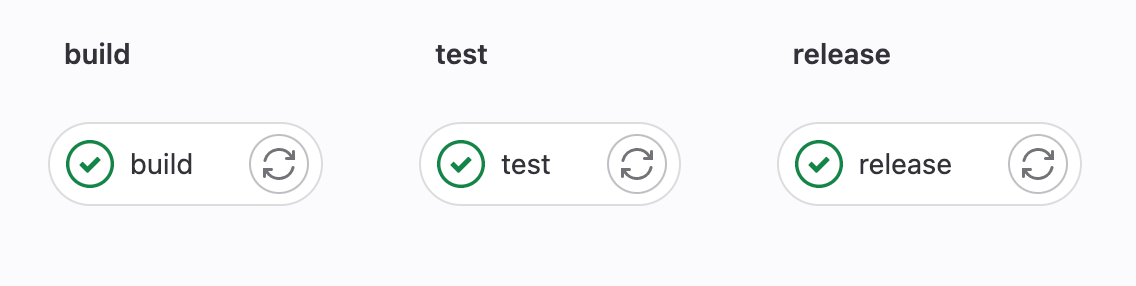
\includegraphics[width=0.8\textwidth]{images/Pipeline.png}
    \caption{Pipeline de la CI}
    \label{fig:gitlab-ci}
\end{figure}

    \chapter{Test unitaires}
\noindent Les tests unitaires sont spécifiques à IntelliJ et permettent de tester les fonctionnalités du plugin.
Ils sont écrits en Java et sont exécutés à chaque commit sur la CI.


\section{Mise en place des tests unitaires}

\noindent Les tests unitaires sont écrits dans le dossier "test" à la racine du projet.
\newdoubleline Ils sont séparés en 2 classes de tests :
\begin{itemize}
    \item \textbf{PrologCodeInsightTest} : Test les fonctionnalités telles que :
    \begin{itemize}
        \item Les annotations
        \item Les commentaires (Line comment, Block comment)
        \item Le renommage par refactoring
        \item La fonction "Find usages"
        \item L'auto-complétion
    \end{itemize}
    \item \textbf{PrologParsingTest} : Test si le parser et le lexer sont correctement générés et fonctionnels.
\end{itemize}

\noindent La classe "PrologCodeInsightTest" étend la classe "LightJavaCodeInsightFixtureTestCase" qui permet de tester les fonctionnalités du plugin de manière plus simple.
\newdoubleline Cette classe permet de configurer des tests automatiques avec des fichiers d'entrée et des fichiers de sortie attendus. Voici un exemple de test :
\begin{lstlisting}
    public void testRenameRefactor() {
        myFixture.configureByFiles("RenameTestData1.pl", "RenameTestData2.pl", "RenameTestData3.pl");
        myFixture.renameElementAtCaretUsingHandler("fifo_new_renamed");
        myFixture.checkResultByFile("RenameTestData1.pl", "RenameTestData1Renamed.pl", false);
        myFixture.checkResultByFile("RenameTestData2.pl", "RenameTestData2Renamed.pl", false);
        myFixture.checkResultByFile("RenameTestData3.pl", "RenameTestData3Renamed.pl", false);
    }
\end{lstlisting}

\noindent La méthode "configureByFiles" permet de charger les fichiers d'entrée.
\\ La méthode "renameElementAtCaretUsingHandler" permet de renommer l'élément sélectionné dans le fichier d'entrée.
\\ La méthode "checkResultByFile" permet de comparer le fichier d'entrée avec le fichier de sortie attendu.

\section{Exécution des tests unitaires}

\noindent Les tests unitaires sont exécutés à chaque commit sur la CI.
\newdoubleline Pour les exécuter en local, il faut lancer la commande suivante :
\begin{lstlisting}
    gradle test
\end{lstlisting}


    \chapter{Ajout des fonctionnalités}


\section{Navigation}
\noindent La navigation est une fonctionnalité très utilisée par les développeurs.
Elle permet de se déplacer dans le code source d'un projet.
Dans le cas d'un projet Prolog, il est important de pouvoir naviguer entre les différents prédicats, leurs usages et leur définitions.
\newdoubleline
Dans le cas d'un language comme Prolog, il est possible de définir plusieurs prédicats avec le même nom mais avec une arité (nombre d'arguments) différente :

\begin{lstlisting}
    predicat(A).
    predicat(A, B).
    predicat(A, B, C).
\end{lstlisting}

La navigation devra donc être consciente de l'arité du prédicat afin de pouvoir naviguer entre les différentes définitions du prédicat mais aussi lors de la recherche de l'utilisation de celui-ci dans le code.
\\ Ceci sera également valable plus tard, lors du refactoring.

\subsection{Goto Declaration}
\noindent Cette partie plus spécifique parlera de la fonctionnalité Goto Declaration.
Cette fonctionnalité permet de naviguer vers la définition d'un prédicat.
Pour cela, il faut sélectionner le prédicat et appuyer sur Ctrl+B (ou Cmd+B sur Mac).
La définition du prédicat s'ouvrira alors dans un nouvel onglet s'il existe.
Si le prédicat est défini à plusieurs endroits, un menu sous forme de popup s'ouvrira et permettra de choisir la définition à ouvrir.
\newdoubleline
\noindent \textbf{Réalisation dans le code}
\\
\noindent La réalisation n'a pas été de tout repos.
En effet, le peu de documentation et d'exemples sur le sujet a rendu la tâche difficile mais finalement réalisable.
\\
\\

\noindent Cheminement:
\begin{enumerate}
    \item Recherche d'exemples sur GitHub et dans la documentation de JetBrains
    \item Création d'une classe \("\)ch.heiafr.intelliprolog.reference.PrologGotoDeclarationHandler\("\)
    \item Méthode de recherche d'inclusion de fichiers
    \item Méthode de recherche des définitions
    \item Méthode qui permet de \("\)matcher\("\) un prédicat avec une définition
\end{enumerate}

\noindent \textbf{Méthode permettant d'extraire le prédicat défini dans la "PrologSentence"}

\begin{lstlisting}[label={lst:method_find_predicate_in_sentence}, caption={Méthode permettant d'extraire le prédicat défini dans la "PrologSentence"}]
public static PsiElement findDefinition(PrologSentence sentence) {

    if (sentence == null) {
        return null;
    }

    //Multiple cases
    Class<?>[][] searchPatterns = new Class[][]{{
            // 1. test :- test2. => atom used as predicate name
            PrologSentence.class, PrologOperation.class, PrologNativeBinaryOperation.class, PrologBasicTerm.class, PrologAtom.class}, {
            // 2. test(A) :- test2. => compound used as predicate name
            PrologSentence.class, PrologOperation.class, PrologNativeBinaryOperation.class, PrologBasicTerm.class, PrologCompound.class}, {
            // 3. test(X). => compound without definition
            PrologSentence.class, PrologCompound.class}, {
            // 4. test. => atom without definition
            PrologSentence.class, PrologAtom.class}};


    for (Class<?>[] searchPattern : searchPatterns) {
        var definition = patternFitPsiElement(sentence, searchPattern);

        if (definition != null) {
            return definition; //Found a definition
        }
    }

    //If not found, return null
    return null;
}
\end{lstlisting}

\noindent Le fonctionnement de cette méthode est le suivant:
\begin{enumerate}
    \item Pour une certaine "PrologSentence" en entrée, on va tester plusieurs cas possibles :
    \begin{enumerate}
        \item test :- test2. => c'est un simple atom qui est défini
        \item test(A) :- test2. => c'est un compound qui est défini
        \item test(X). => c'est un compound qui est défini mais enoncé en tant que fait
        \item test. => c'est un atom qui est défini mais enoncé en tant que fait
    \end{enumerate}
    \item Si le cas est trouvé, on récupère le prédicat correspondant
    \item Sinon, on retourne null
\end{enumerate}
\textbf{Méthode permettant de trouver tous les fichiers inclus récursivement}
\begin{lstlisting}[label={lst:method_find_all_included_files}, caption={Méthode permettant de trouver tous les fichiers inclus récursivement}]
public static Collection<PsiElement> findEveryImportedFile(PsiElement elt, Collection<String> files) {
    if (elt == null) {
        return new ArrayList<>();
    }

    Collection<String> paths = PsiTreeUtil.collectElementsOfType(elt.getContainingFile(), PrologSentence.class).stream()
            .map(ReferenceHelper::findIncludeStatement)// Find the first compound name which is the predicate name
            .filter(Objects::nonNull) //Prevent null values
            .map(ReferenceHelper::extractQuotedString)//Extract the quoted string
            .filter(Objects::nonNull)//Prevent null values
            .filter(s -> !files.contains(s)) //Filter out already visited files
            .collect(Collectors.toList()); //Collect to list

    files.addAll(paths); //Add the new paths to the list of visited files to prevent infinite recursion

    Collection<PsiElement> psiFiles = new ArrayList<>(); //Create a new list of psi files
    for (String path : paths) {
        PsiElement rootElt = pathToPsi(elt, path); //Get the psi element from the path
        psiFiles.add(rootElt); //Add the psi element to the list
        psiFiles.addAll(findEveryImportedFile(rootElt, files)); //Find imported files recursively
    }
    return psiFiles;
}
\end{lstlisting}

\noindent Le fonctionnement de cette méthode est le suivant:
\begin{enumerate}
    \item On recherche toutes les "PrologSentence" du fichier
    \item Pour chaque "PrologSentence", on va chercher le prédicat "include"
    \item Si le prédicat est trouvé, on va chercher le chemin du fichier inclus
    \item Si le chemin n'a pas déjà été visité, on va chercher le fichier correspondant
    \item Si le fichier est trouvé, on va chercher tous les fichiers inclus dans ce fichier de manière récursive
    \item On retourne la liste des fichiers trouvés
\end{enumerate}


\begin{figure}[H]
    \centering
    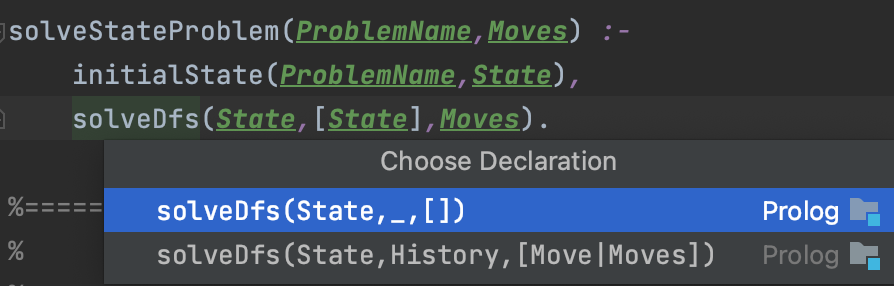
\includegraphics[width=0.8\textwidth]{images/Goto_Declaration.png}
    \caption{Déclaration d'un prédicat}
    \label{fig:definition}
\end{figure}

\subsection{Find usage}
\noindent Pour la recherche d'utilisation, c'est un peu plus simple car certaines méthodes sont déjà implémentées lors de la réalisation du "Goto declaration".
\newdoubleline
En revanche, la recherche doit être exécutée dans un thread séparé pour éviter de bloquer l'IDE pendant la recherche. Si ce n'est pas le cas, une exception est levée automatiquement par l'IDE afin d'interrrompre la méthode.
\newdoubleline
Le fonctionnement est le suivant:
\begin{enumerate}
    \item On récupère le prédicat à rechercher
    \item On lance la recherche dans un thread séparé afin de ne pas bloquer l'IDE
    \item On récupère tous les fichiers .pl
    \item On filtre en fonction de la portée désirée (choisi par l'utilisateur)
    \item On filtre et on retourne les résultats sous forme de UsageInfo
    \item Le Thread s'arrête et les résultats sont affichés
\end{enumerate}

\noindent \textbf{Lancement d'un thread séparé}
\begin{lstlisting}[label={lst:method_find_usages}, caption={Lancement d'un thread séparé}]
public class PrologCustomUsageSearcher extends CustomUsageSearcher {

    @Override
    public void processElementUsages(@NotNull PsiElement element,
                @NotNull Processor<? super Usage> processor, @NotNull FindUsagesOptions options) {

        Application app = ApplicationManager.getApplication(); // get the application

        app.runReadAction(new FindPrologCompoundNameRunnable(element, processor, options));
    }

    private static class FindPrologCompoundNameRunnable implements Runnable {
        private final PsiElement element;
        private final Processor<? super Usage> processor;
        private final FindUsagesOptions options;

        public FindPrologCompoundNameRunnable(PsiElement elt, Processor<? super Usage> processor, FindUsagesOptions options) {
            //Code here
        }

        @Override
        public void run() {
            //Code here
        }
    }
}
\end{lstlisting}

\begin{figure}[H]
    \centering
    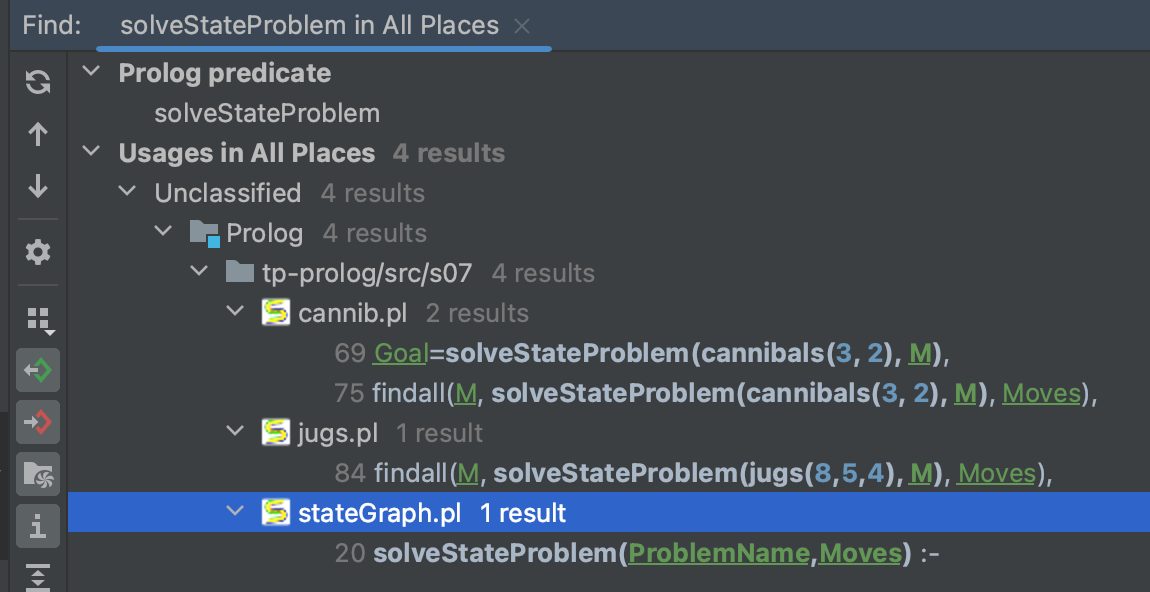
\includegraphics[width=0.8\textwidth]{images/Find_Usage.png}
    \caption{Recherche d'utilisation d'un prédicat}
    \label{fig:usage}
\end{figure}


\section{Refactoring}
\noindent Le refactoring est une fonctionnalité qui permet de modifier le code de manière automatique comme par exemple renommer une variable, une méthode, etc.
C'est une fonctionnalité très appréciée des développeurs car elle permet de gagner du temps et d'éviter les erreurs de frappe ou simplement les oublis lors de la modification du code.
\newdoubleline
Dans notre cas, seul la partie renommage d'un prédicat, d'un atome ou d'une variable nous intéresse.
En effet, il est fréquent de renommer un prédicat ou une variable dans un fichier Prolog et il est important de renommer
toutes les occurrences de ce prédicat ou de cette variable dans tous les fichiers inclus.

\subsection{Renommer un prédicat}
\noindent Pour renommer un prédicat, il faut d'abord récupérer le prédicat à renommer.
Ensuite, il faut récupérer tous les fichiers inclus dans le fichier courant ainsi que tous les fichiers inclus dans ces
fichiers inclus et ainsi de suite.
\newdoubleline
Il faut ensuite remplacer toutes les occurrences du prédicat par le nouveau nom.
\newdoubleline

Exemple d'un renommage de prédicat:

\begin{figure}[H]
    \centering
    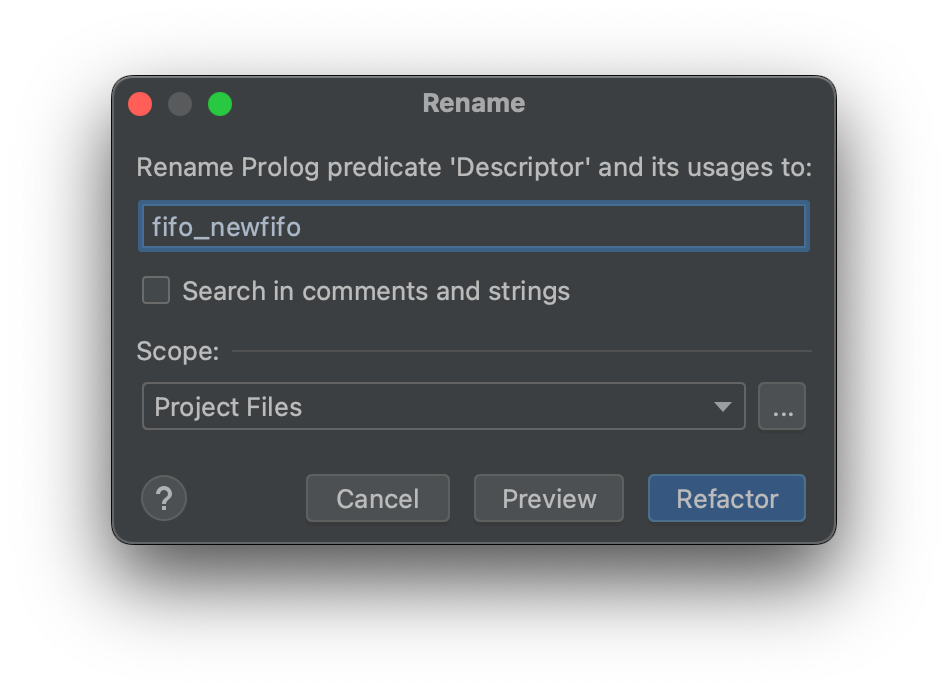
\includegraphics[width=0.8\textwidth]{images/Refactor_window.png}
    \caption{Fenêtre de renommage d'un prédicat}
    \label{fig:refactor_window}
\end{figure}

\begin{figure}[H]
    \centering
    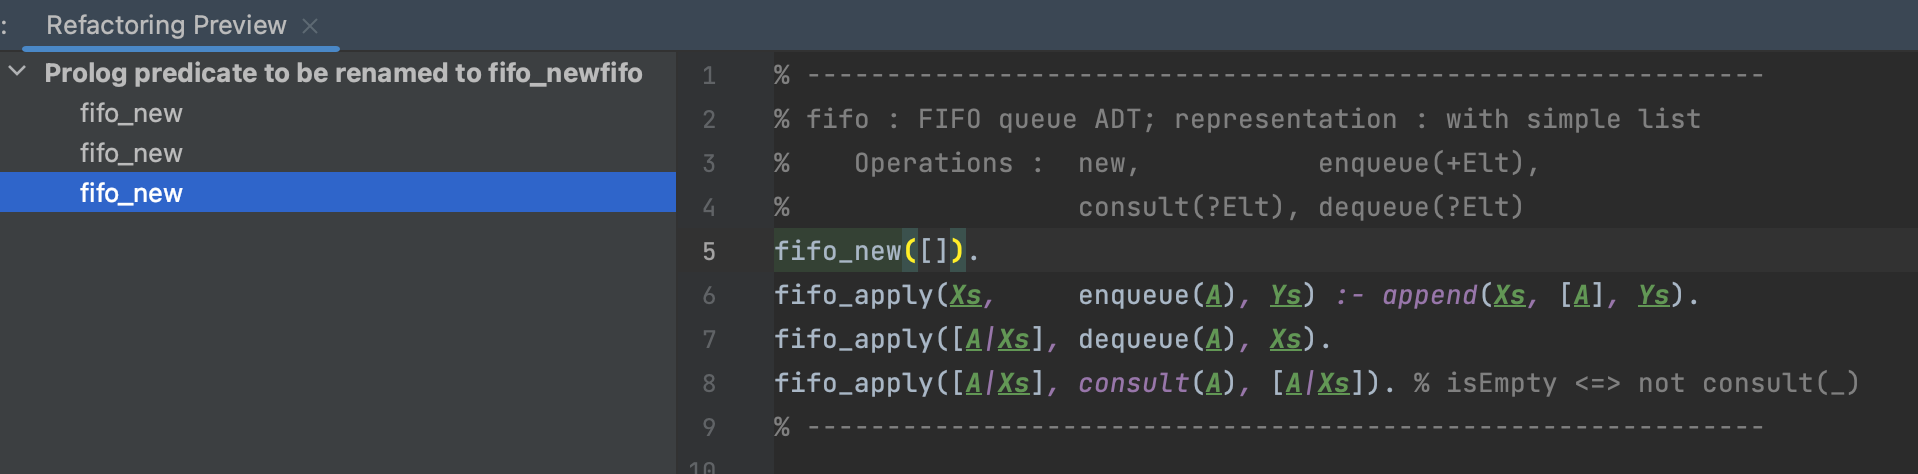
\includegraphics[width=0.8\textwidth]{images/Refactoring_preview.png}
    \caption{Aperçu du refactoring}
    \label{fig:refactor_preview}
\end{figure}

\subsection{Renommer une variable}
\noindent Pour ce qui est du renommage d'une variable, la portée du refactoring est limitée à la phrase Prolog dans laquelle se trouve la variable.
\newdoubleline
Le fonctionnement est similaire à celui du renommage d'un prédicat, à la différence que l'on ne va pas chercher en dehors de la phrase Prolog dans laquelle se trouve la variable.

\subsection{Fonctionnement du renommage}
\noindent Le fonctionnement du renommage est le suivant:
\begin{enumerate}
    \item On récupère le prédicat ou la variable à renommer
    \item On récupère tous les fichiers inclus dans le fichier courant
    \item On récupère tous les fichiers inclus dans ces fichiers inclus et ainsi de suite
    \item On affiche un aperçu des modifications
    \item On remplace toutes les occurrences du prédicat ou de la variable par le nouveau nom
\end{enumerate}

\noindent La classe qui gère le renommage est la suivante \textbf{PrologRenamePsiElementProcessor}.
Voici une brève description des méthodes de cette classe héritée de \textbf{RenamePsiElementProcessor}:
\begin{enumerate}
    \item \textbf{canProcessElement}: Cette méthode permet de vérifier si l'élément peut être renommé. Dans notre cas, on vérifie si l'élément est un prédicat ou une variable.
    \item \textbf{prepareRenaming}: Cette méthode permet de préparer le renommage. Dans notre cas, on récupère tous les prédicats de tous les fichiers touchés par le renommage.
    \item \textbf{renameElement}: Cette méthode permet de renommer chaque prédicat/variable.
\end{enumerate}


\section{Affichage des erreurs et warnings}
\noindent Lors de la compilation d'un fichier Prolog, il est possible que des erreurs ou des warnings apparaissent
qui ne sont pas détectés plus tôt car ce ne sont pas des erreurs de syntaxe.
\newdoubleline
Par exemple, il est possible d'avoir une erreur de prédicats non définis ou une erreur de variables non définies ou simplement des avertissements par rapport à des variables "Singletons".

\subsection{L'idée}
\noindent L'idée est de récupérer les erreurs et les warnings de la compilation du fichier Prolog et de les afficher dans l'éditeur Prolog.
\newdoubleline
Ceci implique différentes contraintes:
\begin{enumerate}
    \item Il faut prendre en compte que la compilation doit avoir lieu en temps réel et en arrière plan.
    \item La compilation doit avoir lieu sur macOS, Linux et Windows.
    Ce qui implique de mettre en place un système multi-plateforme.
    \item La compilation doit aussi être dans un thread séparé pour ne pas bloquer l'interface et ne pas ralentir l'éditeur.
\end{enumerate}

\subsection{La mise en pratique}
\noindent Pour la compilation, nous utiliserons le SDK relatif au projet ouvert.
\newdoubleline
Pour l'aspect compilation en temps réel, JetBrains propose une classe nommée "ExternalAnnotator" qui permet de faire des annotations externes.
\newdoubleline
Cette classe permet de faire des annotations externes, notamment à l'aide d'un thread séparé. La classe se présente comme suit:
\begin{enumerate}
    \item \textbf{collectInformation}: Cette méthode permet de récupérer les informations afin de générer les annotations.
    C'est dans cette partie que le lancement de la compilation aura lieu.
    \item \textbf{doAnnotate}: Cette méthode permet de générer les annotations pour chaque ligne.
\end{enumerate}

\noindent Voici le code permettant de récupérer un processus de compilation Prolog:
\begin{lstlisting}[label={lst:get_prolog_process}, caption={Méthode de créer un processus de compilation Prolog}, language=java]
    public static Process getProcess(Path compiler, Path filePath) throws IOException, CantRunException {
        Process p;
        BufferedWriter writer;

        if (SystemInfo.isWindows) {
            p = Runtime.getRuntime().exec("cmd.exe /min");
            writer = new BufferedWriter(new java.io.OutputStreamWriter(p.getOutputStream()));
            writer.write("set LINEDIT=gui=no"); //Prevent windows from opening a console
            writer.newLine();
            writer.write(compiler.toString()); //Launch the compiler
            writer.newLine();
            writer.flush(); //Flush the stream
        } else {
            p = Runtime.getRuntime().exec(compiler.toString());
            writer = new BufferedWriter(new java.io.OutputStreamWriter(p.getOutputStream()));
        }

        writer = new BufferedWriter(new java.io.OutputStreamWriter(p.getOutputStream()));
        String normalizedFilePath = filePath.toString().replace("\\", "/"); //Mandatory for windows
        String goal = "consult('" + normalizedFilePath + "').";
        writer.write(goal);
        writer.newLine();
        writer.flush();
        writer.close();
        return p;
    }
\end{lstlisting}

\noindent Au final, voici le résultat en action dans l'éditeur :
\begin{figure}[h]
    \centering
    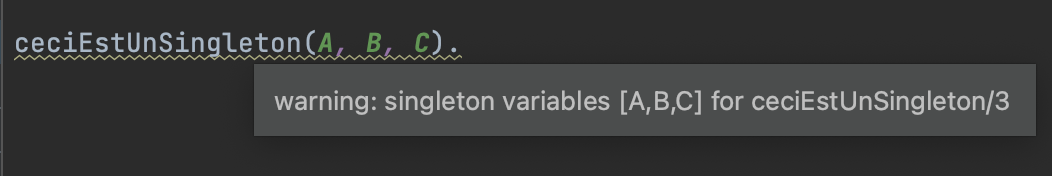
\includegraphics[width=0.8\textwidth]{images/background_compilation.png}
    \caption{Affichage d'avertissement grâce à la compilation}
    \label{fig:compilation_warnings}
\end{figure}

\section{Auto-complétion}


\section{Formatage du code}


\section{Déploiement du plugin}

    \chapter{Déploiement}
\noindent Nous avons décider de déployer le plugin sur le marketplace de Jetbrains.
Afin de permettre à tout le monde de pouvoir modifier le plugin, nous avons aussi décider de le mettre sur Github.


\section{Choix de la licence}
\noindent Nous avons choisi de mettre le plugin sous la licence MIT car elle est très permissive et permet à tout le monde de pouvoir modifier le plugin.
Une licence moins permissive aurait pu être la GNU GPLv3, mais elle impose de mettre le code source en open source et de mettre la licence dans le plugin.
\newdoubleline Voici un tableau comparatif des différentes licenses que nous avons étudié :

\begin{table}[H]
    \begin{tabular}{lccccc}
        \textbf{Permissions}    & \multicolumn{1}{l}{MIT} & \multicolumn{1}{l}{GNU GPLv3} & \multicolumn{1}{l}{GNU LGPLv3} & \multicolumn{1}{l}{Mozilla Public 2.0} & \multicolumn{1}{l}{Apache 2.0} \\
        Utilisation commerciale & x                               & x                             & x                              & x                                              & x                                      \\
        Utilisation privée      & x                               & x                             & x                              & x                                              & x                                      \\
        Distribution            & x                               & x                             & x                              & x                                              & x                                      \\
        Modification            & x                               & x                             & x                              & x                                              & x                                      \\
        \textbf{Conditions}     &                                 &                               &                                &                                                &                                        \\
        Indiquer la source      &                                 & x                             & x                              & x                                              &                                        \\
        Même licence            &                                 & x                             & x                              & x                                              &                                        \\
        \begin{tabular}[c]{@{}l@{}}
            Indiquer la licence \\ et le copyright
        \end{tabular} & x & x & x & x & x
    \end{tabular}
\end{table}

\section{Déploiement sur le marketplace}
\noindent Pour déployer le plugin sur le marketplace, il faut créer un compte sur le site de Jetbrains.
Une fois le compte créé, il suffit de se rendre sur la page de déploiement du plugin, de choisir le plugin à déployer et de remplir les informations demandées.
\newdoubleline Voici un exemple de ce que l'on peut voir sur la page de déploiement du plugin :

\begin{figure}[H]
    \centering
    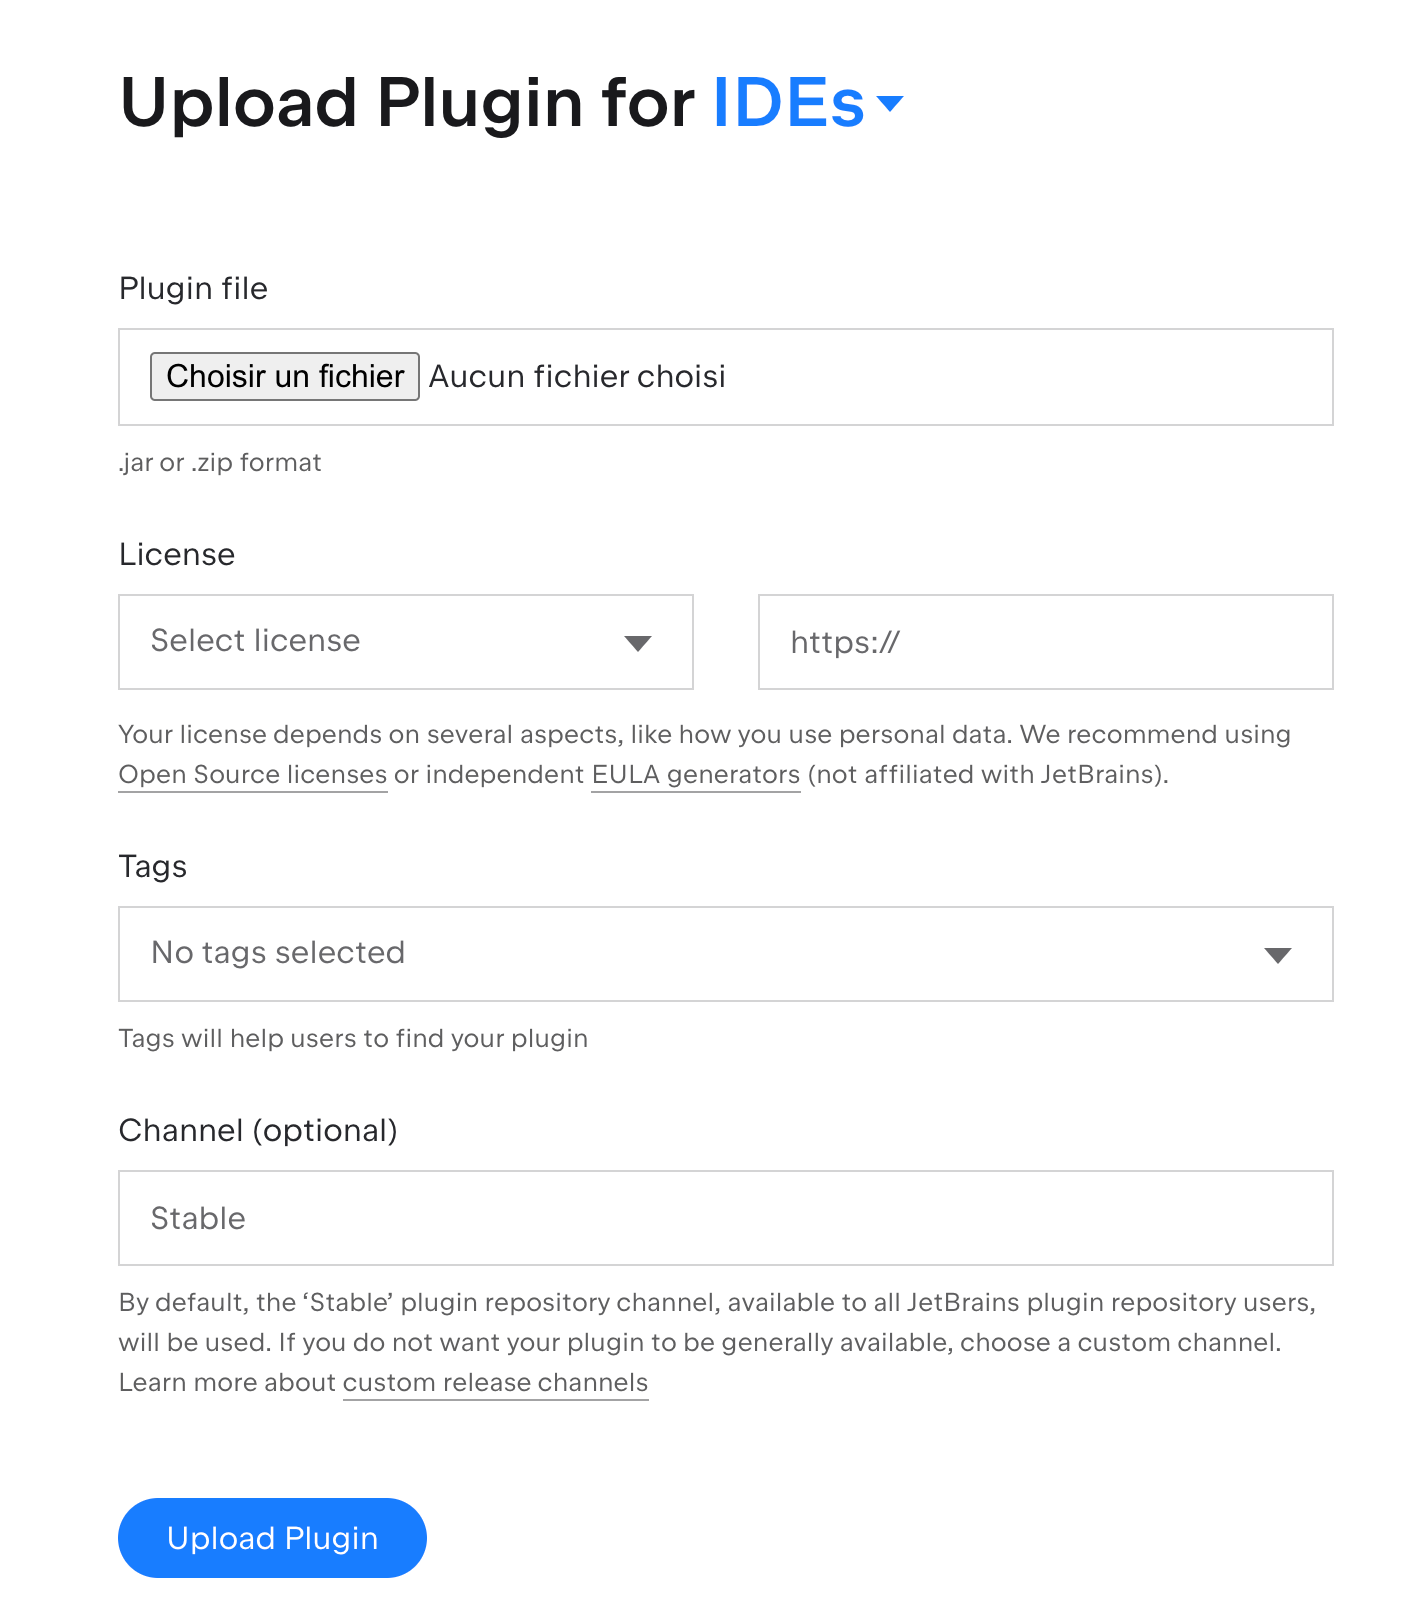
\includegraphics[width=0.5\textwidth]{images/first_deploy.png}
    \caption{Premier déploiement du plugin}
    \label{fig:first_deploy}
\end{figure}

\noindent Lors des déploiements suivants, il suffit de cliquer sur le bouton « Update » et de choisir le fichier .zip du plugin.
\newdoubleline La page du plugin sur le marketplace est la suivante : \url{https://plugins.jetbrains.com/plugin/20922-intelliprolog}

\section{Déploiement sur Github}
\noindent Une organisation Github a été créée pour le projet.
Le projet a été publié à l'adresse suivante: \url{https://github.com/IntelliProlog/IntelliProlog}



    \chapter{Conclusion}

    
    \printnoidxglossary[title=Glossaire,nonumberlist]
   
    
    
    % table of figures
    {
    \let\oldnumberline\numberline%
    \renewcommand{\numberline}{\figurename~\oldnumberline}%
    \renewcommand{\listfigurename} {Table des illustrations}
    \newpage
    \listoffigures%
    
    \renewcommand{\numberline}{\listingsname~\oldnumberline}%
    \newpage
    \addcontentsline{toc}{chapter}{Liste des codes}
    \lstlistoflistings
    }


    
    % add bibliography
    \bibliographystyle{alphabetic}
    \bibliography{bibliography}
    
\end{document}